\documentclass[border=0pt]{standalone}
\usepackage{amsmath}
\usepackage{mathptmx}
\usepackage{tikz}
\usetikzlibrary{arrows.meta, calc, patterns.meta, backgrounds}

\definecolor{otblue}{HTML}{0072B2}
\definecolor{otorange}{HTML}{E69F00}
\definecolor{otteal}{HTML}{009E73}
\definecolor{otpurple}{HTML}{CC79A7}
\definecolor{otgray}{HTML}{5A5A5A}

\def\unit{1.34}      % width of one unit of running time, cm
\def\lane{0.40}      % bar height, cm
\def\gap{0.09}       % gap between lanes, cm
\def\panelh{1.56}    % panel height, cm
\def\panelgap{0.12}  % gap between panels, cm
\def\left{-0.98}     % left edge of a panel, cm
\def\right{7.58}     % right edge of a panel, cm
\def\note{2.95}      % left edge of the outcome column, cm

\tikzset{
  bar/.style={rounded corners=1.6pt, line width=0.55pt, inner sep=0pt, font=\scriptsize, align=center,
              minimum height=\lane cm},
  alice/.style={bar, draw=otblue!75!black, fill=otblue, text=white},
  bob/.style={bar, draw=otorange!70!black, fill=otorange!45, text=black},
  held/.style={bar, draw=otblue!75!black, dash pattern=on 2pt off 1.2pt},
  hatch/.style={rounded corners=1.6pt, pattern={Lines[angle=45,distance=2.4pt,line width=0.45pt]}, pattern color=otblue!55},
  soft/.style={rounded corners=1.6pt, draw=otblue!75!black, dash pattern=on 0.8pt off 1.1pt, line width=0.6pt},
  lanelabel/.style={font=\scriptsize, text=otgray!85!black, anchor=east, inner sep=0pt},
  title/.style={font=\footnotesize\bfseries, text=black, anchor=north west, inner sep=0pt},
  outcome/.style={font=\scriptsize, text=black, anchor=west, inner sep=0pt, align=left, text width=4.55cm},
  aside/.style={font=\scriptsize\itshape, text=otblue!75!black, anchor=west, inner sep=0pt},
}

\newcommand{\panel}[3]{%
  \fill[#2, rounded corners=3pt] (\left,#1) rectangle (\right,{#1+\panelh});
  \node[title] at (\left+0.14,{#1+\panelh-0.09}) {#3};
  \node[lanelabel] at (-0.08,{#1+0.10+\lane+\gap+\lane/2}) {Alice};
  \node[lanelabel] at (-0.08,{#1+0.10+\lane/2}) {Bob};
}
\newcommand{\gantt}[6]{%
  \node[#5, minimum width={(#4-#3)*\unit cm}, anchor=south west] at ({#3*\unit},{#1+0.10+#2*(\lane+\gap)}) {#6};}

\begin{document}
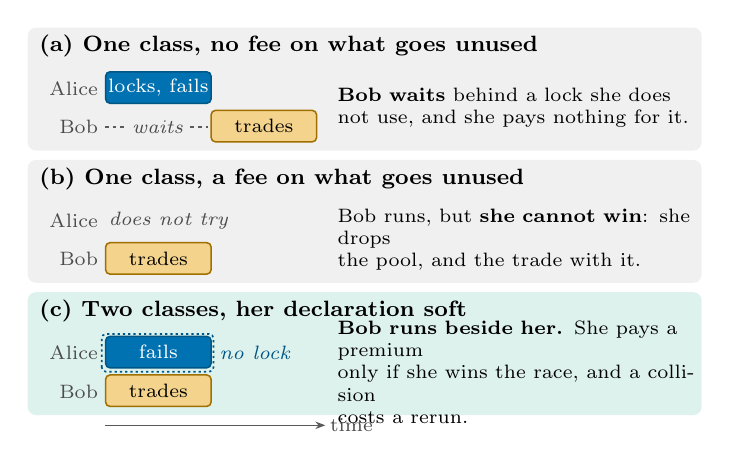
\begin{tikzpicture}
  \pgfmathsetmacro{\ya}{2*(\panelh+\panelgap)}
  \pgfmathsetmacro{\yb}{\panelh+\panelgap}
  \pgfmathsetmacro{\yc}{0}

  \panel{\ya}{otgray!9}{(a) One class, no fee on what goes unused}
  \gantt{\ya}{1}{0}{1}{alice}{locks, fails}
  \gantt{\ya}{0}{1}{2}{bob}{trades}
  \draw[held, dash pattern=on 1.4pt off 1.4pt, line width=0.45pt, draw=otgray] (0,{\ya+0.10+\lane/2}) -- (\unit-0.03,{\ya+0.10+\lane/2});
  \node[font=\scriptsize\itshape, text=otgray!85!black, fill=otgray!9, inner xsep=2pt, inner ysep=0.2pt] at ({0.5*\unit},{\ya+0.10+\lane/2}) {waits};
  \node[outcome] at (\note,{\ya+0.10+\lane+\gap/2}) {\textbf{Bob waits} behind a lock she does\\not use, and she pays nothing for it.};

  \panel{\yb}{otgray!9}{(b) One class, a fee on what goes unused}
  \node[aside, text=otgray!85!black] at (0.04,{\yb+0.10+\lane+\gap+\lane/2}) {does not try};
  \gantt{\yb}{0}{0}{1}{bob}{trades}
  \node[outcome] at (\note,{\yb+0.10+\lane+\gap/2}) {Bob runs, but \textbf{she cannot win}: she drops\\the pool, and the trade with it.};

  \panel{\yc}{otteal!13}{(c) Two classes, her declaration soft}
  \gantt{\yc}{1}{0}{1}{alice}{fails}
  \draw[soft] (-0.04,{\yc+0.10+\lane+\gap-0.04}) rectangle ({\unit+0.04},{\yc+0.10+2*\lane+\gap+0.04});
  \node[aside] at ({\unit+0.11},{\yc+0.10+\lane+\gap+\lane/2}) {no lock};
  \gantt{\yc}{0}{0}{1}{bob}{trades}
  \node[outcome] at (\note,{\yc+0.10+\lane+\gap/2}) {\textbf{Bob runs beside her.} She pays a premium\\only if she wins the race, and a collision\\costs a rerun.};

  \draw[-{Stealth[length=3.6pt]}, line width=0.45pt, draw=otgray] (0,-0.13) -- ({2*\unit+0.12},-0.13);
  \node[font=\scriptsize, text=otgray!85!black, anchor=west, inner sep=1.5pt] at ({2*\unit+0.12},-0.13) {time};
\end{tikzpicture}
\end{document}
